% Build from the repository root with latexmk or make.
% Shared document class, packages, and formatting for LuaLaTeX.
% Based on the TUDoThesis template by Maximilian Nöthe; see LICENSE.
\documentclass[
  tucolor,               % Remove for headings without TU green.
  BCOR=12mm,             % Adjust the binding correction for the final binding.
  parskip=half,
  open=any,
  cleardoublepage=plain,
]{tudothesis}

\setcounter{tocdepth}{1} % List chapters and sections in the contents.
\usepackage[aux]{rerunfilecheck}

% Fonts and languages. The last Babel language is the main language.
\usepackage{fontspec}
\defaultfontfeatures{Ligatures=TeX}
\usepackage[ngerman, american]{babel}
\usepackage[autostyle]{csquotes}
\usepackage{microtype}

% Mathematics. unicode-math supplies the symbols formerly loaded by amssymb.
\usepackage{mathtools}
\usepackage[
  math-style=ISO,
  bold-style=ISO,
  sans-style=italic,
  nabla=upright,
  partial=upright,
  warnings-off={mathtools-colon,mathtools-overbracket},
]{unicode-math}
\setmathfont{Latin Modern Math}
\usepackage{xfrac}

% Numbers and units follow the active document language.
\usepackage[
  locale=US,
  separate-uncertainty=true,
  per-mode=symbol-or-fraction,
]{siunitx}
\addto\extrasamerican{\sisetup{locale=US}}
\addto\extrasngerman{\sisetup{locale=DE}}

% Tables and graphics. Caption/subcaption support is provided by tudothesis.
\usepackage{booktabs}
\usepackage{graphicx}
\graphicspath{{figures/}{plots/}{logos/}}
\usepackage{scrhack}
\usepackage{float}
\floatplacement{figure}{htbp}
\floatplacement{table}{htbp}
\usepackage[section, below]{placeins}
\usepackage{pdfpages}
\pdfvariable minorversion=7

\usepackage{enumitem}
\setlist{nolistsep}
\usepackage[shortcuts]{extdash}

% Each document declares its own .bib resource after loading this header.
\usepackage[
  backend=biber,
  autolang=hyphen,
]{biblatex}

% Load hyperlink support near the end, before bookmarks and glossaries.
\usepackage[
  unicode,
  colorlinks=true,
  linkcolor=tugreen!55!black,
  citecolor=tugreen!55!black,
  urlcolor=blue!70!black,
]{hyperref}
\usepackage{bookmark}
\usepackage[toc, acronym]{glossaries}
\makenoidxglossaries % Uses LaTeX reruns; no external indexer is required.

% Reusable notation belongs here; package and layout settings belong in header.tex.
% Bold italic vectors, using unicode-math's ISO-style alphabet.
\newcommand{\vect}[1]{\symbf{#1}}

% Edit the thesis details here. Bracketed fields are placeholders.
\newcommand{\thesisauthor}{Akram Aki}
\author{\thesisauthor}
\title{[Master's thesis title]}
\date{2027} % Year shown on the title page.
\birthplace{Hagen}
\chair{Research Group Rhode / Elsässer} % Confirm the group for this thesis.
\division{Faculty of Physics}
\thesisclass{Master of Science}
\submissiondate{[Submission date]}
\firstcorrector{[Primary reviewer]}
\secondcorrector{[Secondary reviewer]}
\titlehead{
\includegraphics[height=1.5cm]{logos/tu-logo.pdf}}

% Set the author explicitly: the class adds the birthplace to the printed author.
\hypersetup{
  pdftitle={\thetitle},
  pdfauthor={\thesisauthor},
  pdfsubject={Master's thesis},
}

\addbibresource{references.bib}
% !TeX root = ../thesis.tex
% Define thesis-specific acronyms and terms here, then use \gls{key} in the text.
% Only entries used in the document are printed. See examples/glossary.tex.


\begin{document}
\frontmatter
\maketitle
\makecorrectorpage

% !TeX root = ../thesis.tex
\begin{otherlanguage}{american}
\chapter*{Abstract}
% Summarize the motivation, methods, main results, and conclusions in English.
\end{otherlanguage}

% !TeX root = ../thesis.tex
\begin{otherlanguage}{ngerman}
\chapter*{Kurzfassung}
% Fasse Motivation, Methoden, wichtigste Ergebnisse und Schlussfolgerungen zusammen.
\end{otherlanguage}


\begingroup
  \hypersetup{hidelinks}
  \tableofcontents
\endgroup
% Enable these if useful once figures and tables have been added:
% \listoffigures
% \listoftables

\mainmatter
% !TeX root = ../thesis.tex
\chapter{Introduction}
\label{ch:introduction}

% Introduce the motivation, research question, and structure of the thesis.

% !TeX root = ../thesis.tex
\chapter{Background}
\label{ch:background}

% Establish the theoretical context and discuss relevant previous work.

% !TeX root = ../thesis.tex
\chapter{Methods}
\label{ch:methods}

% Describe the methods, data or experimental setup, and validation strategy.

% !TeX root = ../thesis.tex
\chapter{Analysis}
\label{ch:analysis}

% Explain the analysis procedure, selection criteria, and uncertainty treatment.

% !TeX root = ../thesis.tex
\chapter{Results}
\label{ch:results}

% Present and interpret the results, including comparisons and limitations.

% !TeX root = ../thesis.tex
\chapter{Conclusion}
\label{ch:conclusion}

\section{Summary}
% Answer the research question and summarize the main contributions.

\section{Outlook}
% Identify open questions and useful directions for future work.


\appendix
% !TeX root = ../thesis.tex
\chapter{Supplementary Material}
\label{app:supplementary}

% Add supporting derivations, supplementary results, or configuration details.


\backmatter
\printnoidxglossaries
\printbibliography
% Adapt this optional section before enabling it:
% % !TeX root = ../thesis.tex
% Optional section: adapt it to actual tool use and applicable requirements,
% then enable its \input in thesis.tex. It is excluded from the default build.
\addchap{Use of AI Tools}
% Describe which tools were used, for which tasks, and how their output was checked.
%
% Bachelor wording retained as an example, not as a statement about this thesis:
% Einzelne Formulierungen dieser Arbeit wurden mit Unterstützung von ChatGPT
% (OpenAI) überarbeitet. Wissenschaftliche Inhalte, Auswertungen und
% Schlussfolgerungen liegen vollständig bei der Autorin/dem Autor; für verbleibende
% Fehler trägt die Autorin/der Autor die Verantwortung.

% !TeX root = ../thesis.tex
% Retained blank form: check the current university/faculty requirements before
% submission and replace this PDF with the completed declaration as appropriate.
% Source: https://www.tu-dortmund.de/studierende/im-studium/pruefungsangelegenheiten/allgemeine-vordrucke/
\cleardoublepage
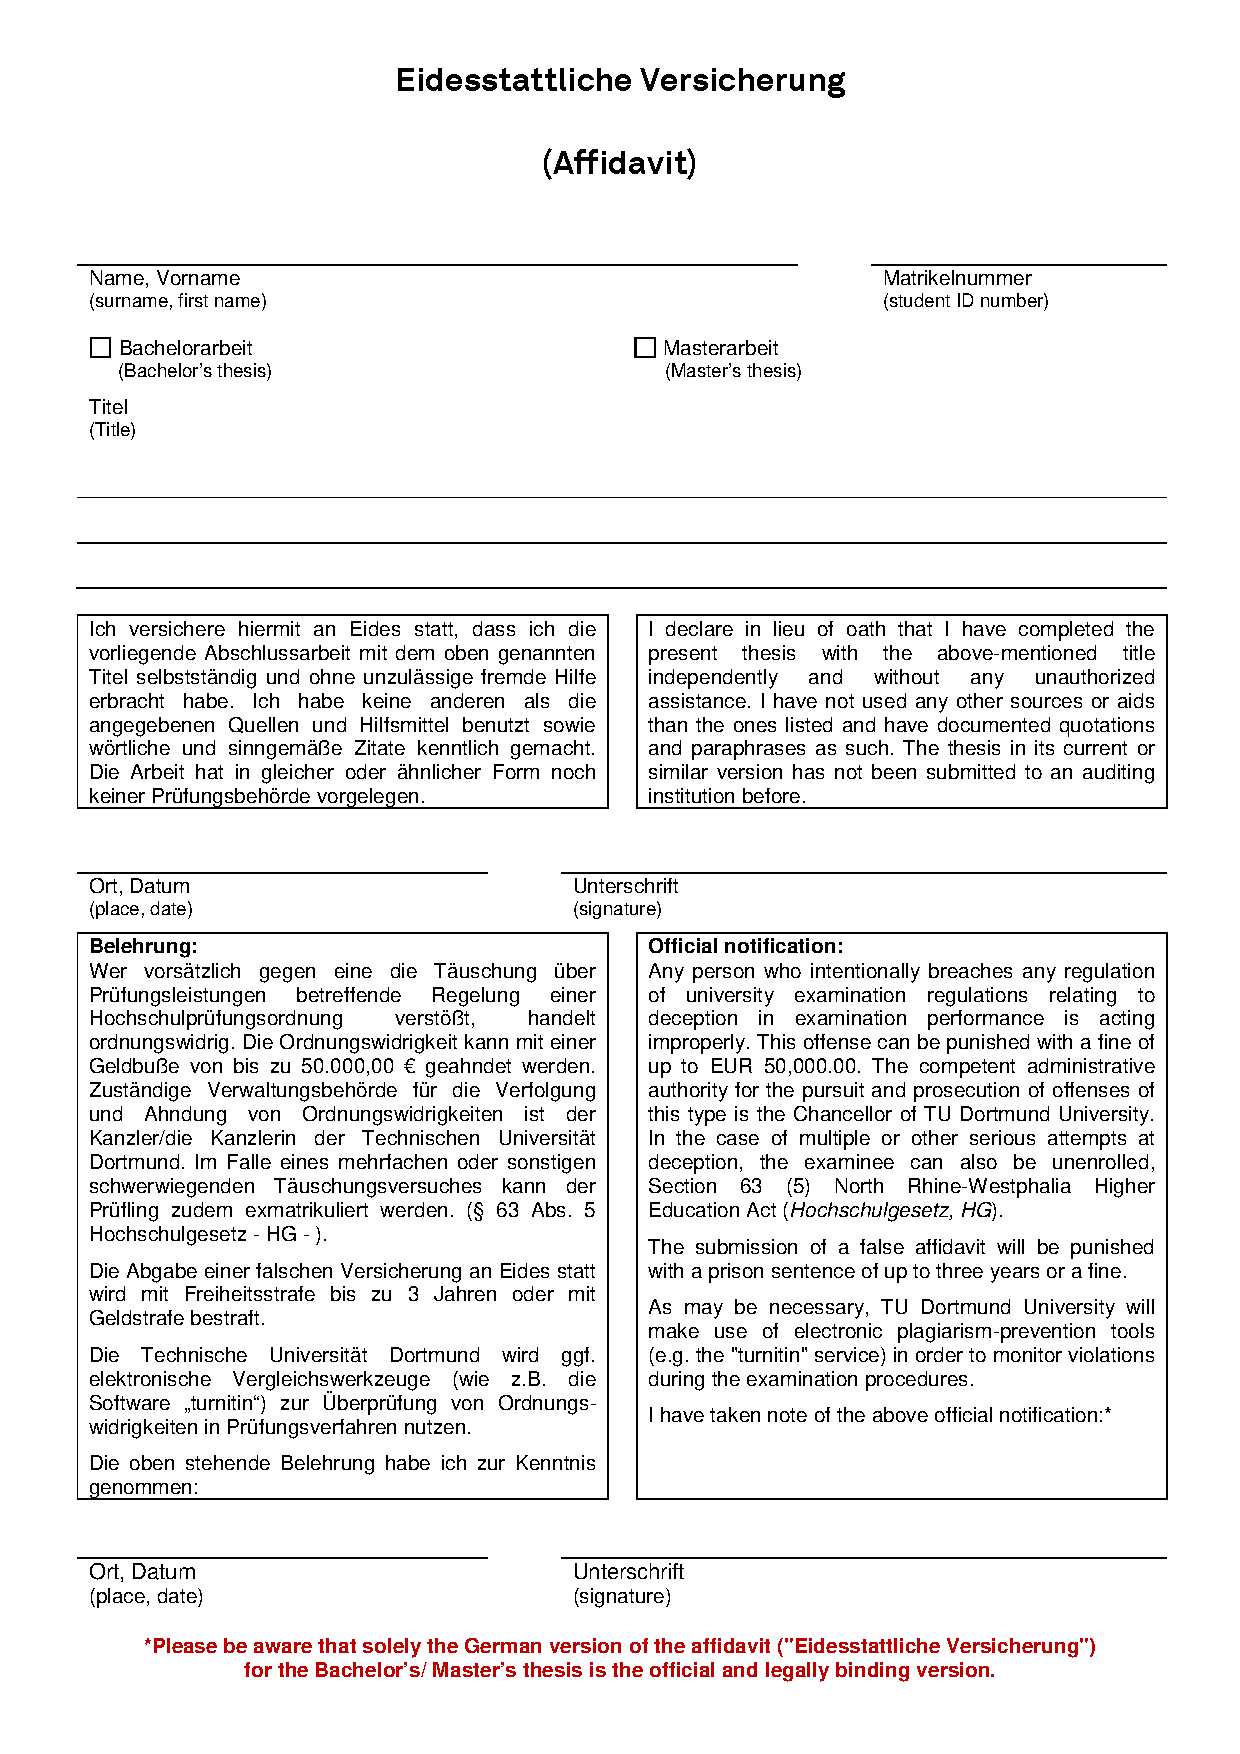
\includepdf[pages=-]{content/Eidesstattliche_Versicherung_original.pdf}


\end{document}
